\section{Experiments}
\label{sec:experiments}

\paragraph{Design.} Ten polynomial systems on $\R^2$ and $\R^3$ serve as
benchmarks: four with a nonzero symmetry algebra inside the affine candidate
class (a Hopf normal form, a planar rotationally symmetric linear system, the
Euler equations of a symmetric top, and a radial flow onto the sphere with full
$\mathfrak{so}(3)$), and six with none (Van der Pol, Duffing,
Lotka--Volterra, Sel'kov, an asymmetric rigid body, and Lorenz). Every system has
rational coefficients, so its exact symmetry algebra is the exact rational
nullspace of the bracket map, computed with symbolic arithmetic; the true defect
of any generator is likewise available in closed form from monomial moments.
\textbf{Ground truth involves no tolerance and no sampling}, which matters here
because the quantity being estimated is itself a near-degeneracy. The exact
algebra dimensions are cross-checked against an independent characterisation
(for linear systems, the dimension of the commutant of the coefficient matrix).

We measure two things, identically for every method. \emph{False certification}
is the event that the declared subspace contains a generator whose true defect
exceeds $\delta$; because the declared object is a subspace, this is evaluated as
a generalised eigenvalue of the true forms restricted to it, not by sampling
directions. \emph{Detection} is the event that the declared dimension is at
least the true one. Unless stated otherwise $\delta = \alpha = 0.05$.

\paragraph{Methods compared, and how we try to be fair to them.} The framework
we build on does not prescribe a tolerance --- it establishes that the symmetries
are a nullspace --- so there is no single baseline to compare against, and we
sweep the tolerance instead of picking one. We also give the threshold rule the
advantage of the \emph{exact} target-domain Gram matrix in
\Cref{sec:calibration}, which no practitioner without our construction would
have; that isolates the purely statistical question and removes the coverage
effect, which is studied separately in \Cref{sec:coverage}. The methods are
(i) a fixed threshold on the plug-in defect, swept
over $\tau \in [0.005, 0.4]$; (ii) the largest relative
eigengap; (iii) a Wald rank test for the nullspace dimension in the spirit of
\citet{robin2000tests} and \citet{kleibergen2006generalized}; (iv) a
split-sample significance test that selects a direction on one half and tests
$H_0$: exact symmetry on the other, declaring a symmetry when it fails to
reject; (v) a Weyl-inequality certificate, the natural singular-value
perturbation answer; (vi) \symcert; (vii) \symcert{} with sample splitting and
the tighter pointwise bound. Full definitions are in \Cref{app:baselines}.

\begin{figure}[t]
\centering
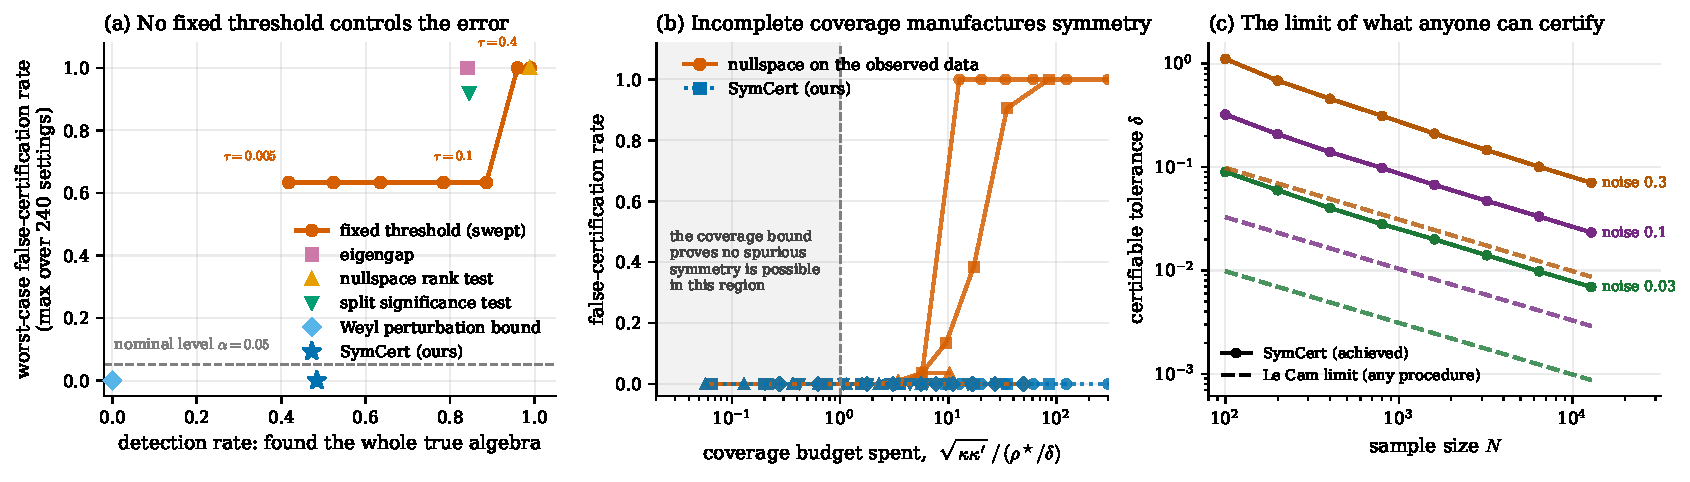
\includegraphics[width=\textwidth]{../figures/fig1_headline.pdf}
\caption{\textbf{(a)} Every method is placed by how often it finds the whole
true symmetry algebra (horizontal) against the largest false-certification rate
it produces over the $240$ settings (vertical). The orange curve traces the
fixed-threshold rule as the tolerance is swept from $0.005$ to $0.4$: no choice
of tolerance brings its worst case near the nominal level (dashed). The rank
test and the split-sample significance test are valid level-$0.05$ tests, and
are among the worst discovery rules, because failing to reject ``this is a
symmetry'' is read as evidence for it. \symcert{} is at $0$; the Weyl
perturbation bound is also at $0$ but never certifies anything.
\textbf{(b)} Shrinking the region the data occupy while keeping the claim about
the full domain. The horizontal axis is the extrapolation bound of
\Cref{prop:kappa} divided by the value it must reach before a spurious
symmetry is arithmetically possible. In the shaded region the proposition
\emph{proves} no spurious symmetry can occur, and none does in any of the $13$
settings there; beyond it the nullspace rule fails on $14$ of $37$ settings.
\symcert{} (blue) is at zero throughout, declining to certify rather than
certifying wrongly. \textbf{(c)} The tolerance that can be certified about a
truly symmetric system, against the Le~Cam limit of \Cref{prop:lecam} for any
procedure with the same error control. Both scale as $\sigma/\sqrt N$; the gap
is a constant factor of $8.1$--$8.8$.}
\label{fig:headline}
\end{figure}

\begin{figure}[t]
\centering
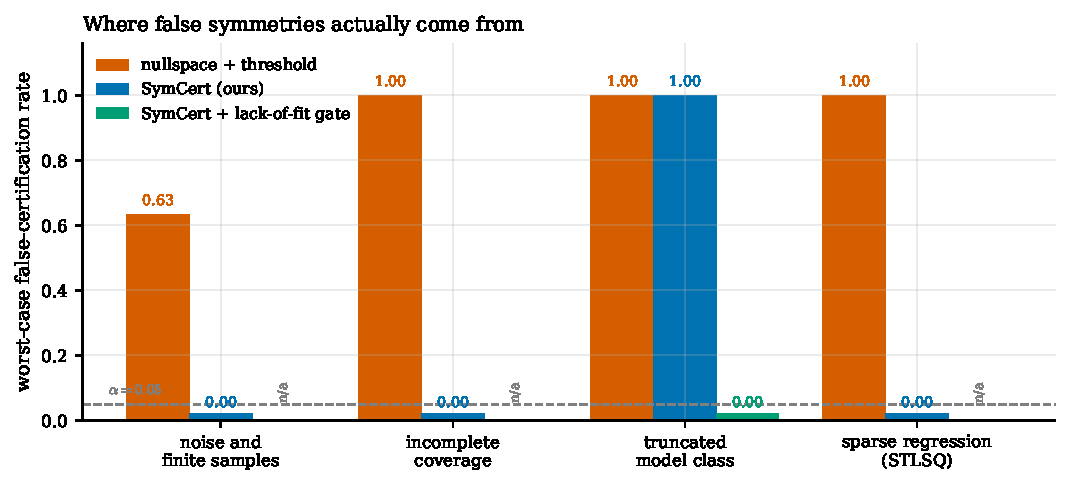
\includegraphics[width=0.72\textwidth]{../figures/fig2_mechanisms.pdf}
\caption{Worst-case false-certification rate under each of the four candidate
mechanisms, at tolerance $\delta = 0.05$. Noise and finite samples alone are the
mildest; incomplete coverage and, above all, the model class are what
manufacture symmetry. \symcert{} controls the first two by construction. It does
\emph{not} control the third, because its validity is conditional on the model
class containing the truth --- but a lack-of-fit test detects every truncated
class we tried and restores control (green). The fourth group is sparse
regression on a weakly symmetry-breaking system: the sparsity threshold deletes
the term that breaks the symmetry, and the resulting model is exactly symmetric.
Certifying from the unpruned fit gives a rate of zero.}
\label{fig:mechanisms}
\end{figure}

\begin{figure}[t]
\centering
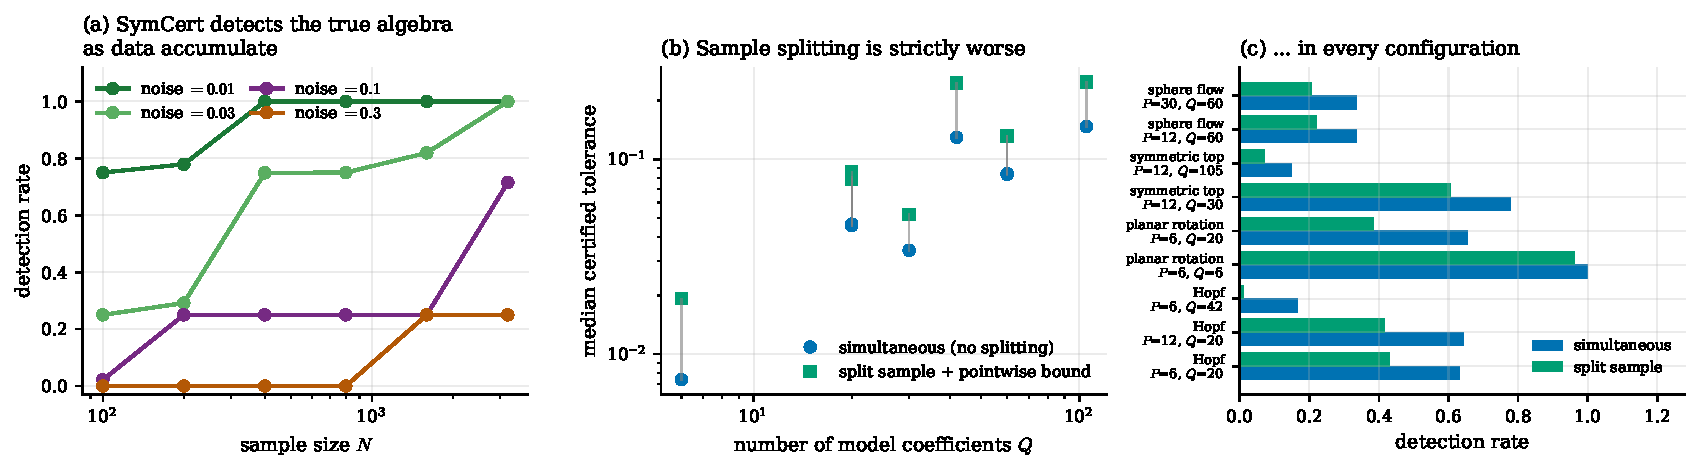
\includegraphics[width=\textwidth]{../figures/fig3_power.pdf}
\caption{\textbf{(a)} The price of validity is detection power, and it is paid
in sample size: at noise level $0.01$ \symcert{} recovers the full true algebra
in every replication from $N = 400$; at noise level $0.3$ it does not, because
the data do not support the claim. \textbf{(b,c)} Simultaneity versus sample
splitting. Each point in (b) is one model configuration; the simultaneous
certificate (blue) is narrower than the split-sample certificate (green) in all
nine, by factors of $1.5$ to $2.6$, and (c) its detection rate is higher in all
nine. Splitting protects against a selection effect that simultaneity already
removes, and pays for that protection with half the data.}
\label{fig:power}
\end{figure}

\subsection{Calibration and power}
\label{sec:calibration}

\Cref{fig:headline}(a) summarises $240$ settings ($10$ systems $\times$ $6$
sample sizes $\times$ $4$ noise levels, $300$ replications each; $72{,}000$
replications in total).

\begin{table}[t]
\centering\small
\begin{tabular}{lrrrr}
\toprule
& \multicolumn{2}{c}{false certification} & detection & \\
\cmidrule(lr){2-3}
method & mean & worst setting & mean & settings above $\alpha$ \\
\midrule
fixed threshold $\tau=0.005$ & 0.005 & 0.633 & 0.418 & 3 / 240 \\
fixed threshold $\tau=0.01$ & 0.005 & 0.633 & 0.523 & 3 / 240 \\
fixed threshold $\tau=0.02$ & 0.005 & 0.633 & 0.635 & 3 / 240 \\
fixed threshold $\tau=0.05$ & 0.005 & 0.633 & 0.784 & 3 / 240 \\
fixed threshold $\tau=0.1$ & 0.017 & 0.633 & 0.886 & 18 / 240 \\
fixed threshold $\tau=0.2$ & 0.139 & 1.000 & 0.960 & 52 / 240 \\
fixed threshold $\tau=0.4$ & 0.551 & 1.000 & 0.990 & 142 / 240 \\
largest eigengap & 0.650 & 1.000 & 0.842 & 166 / 240 \\
nullspace rank test & 0.070 & 1.000 & 0.988 & 30 / 240 \\
split significance test & 0.070 & 0.920 & 0.845 & 37 / 240 \\
Weyl perturbation bound & 0.000 & 0.000 & 0.000 & 0 / 240 \\
\midrule
\symcert{} (ours) & \textbf{0.000} & \textbf{0.000} & 0.484 & \textbf{0 / 240} \\
\symcert{} + sample splitting & \textbf{0.000} & \textbf{0.000} & 0.370 & \textbf{0 / 240} \\
\bottomrule
\end{tabular}
\caption{Calibration and power over 240 settings, 300 replications each. ``Worst setting'' is the
maximum false-certification rate over the settings; the last column counts those
exceeding the nominal $\alpha = 0.05$. No fixed threshold controls the error,
and the two significance-test procedures --- both valid tests --- are the worst
offenders relative to their apparent rigour. The Weyl certificate is valid but
never certifies anything.}
\label{tab:calibration}
\end{table}


Three readings of \Cref{tab:calibration}.

\emph{No fixed threshold is safe.} Lowering $\tau$ does not fix the problem: even
at $\tau = 0.005$ the worst setting has a $63\%$ false-certification rate, while
detection has already fallen to $0.42$. The offending settings are the
\emph{symmetric} systems at high noise, where the threshold recovers the right
\emph{dimension} but the wrong \emph{subspace} --- the selected eigenvectors have
rotated away from the true algebra. A metric that only counted dimensions would
miss this entirely.

\emph{Valid tests are not safe either.} The rank test and the split-sample
significance test are correct level-$0.05$ tests of ``this is an exact
symmetry''. Used as discovery rules they reach false-certification rates of
$1.00$ and $0.92$. This is the inverted burden of proof made quantitative: their
power is lowest exactly where the data are least informative, and low power is
read as evidence for symmetry.

\emph{The tolerance is a choice, and it changes what is at stake.}
\Cref{fig:tolerance} repeats the comparison across $\delta \in [0.01, 0.4]$ on a
smaller grid --- six systems, two sample sizes, two noise levels. \symcert{}'s
worst-case error is zero at every tolerance, and its detection rate climbs from
$0.25$ at $\delta = 0.01$ to $1.00$ at $\delta = 0.2$: a user who will accept a
$20\%$ relative defect can have both error control and full detection here, and
one who insists on $1\%$ cannot. The threshold rule's worst case is $0.50$ at
$\delta = 0.01$ and below the nominal level at the other five values. That is
not a defence of it. On this smaller and easier grid it happens to be safe at
most tolerances; on the full grid of \Cref{tab:calibration} its worst case is
$0.63$ at every $\tau$ we tried. Which of those two situations one is in is
precisely what a threshold cannot tell you, and what the certificate can.

\emph{Validity is not free, and neither is it vacuous.} \symcert{} never errs, at
a detection cost relative to a threshold at the same tolerance ($0.48$ against
$0.78$). \Cref{fig:power}(a) shows where the cost falls: at noise level $0.01$
detection reaches $1.00$ by $N = 400$; at noise level $0.30$ it does not, because
--- correctly --- the data at that noise level do not support the claim. The Weyl
certificate shows the alternative failure: valid, and useless.

\begin{figure}[t]
\centering
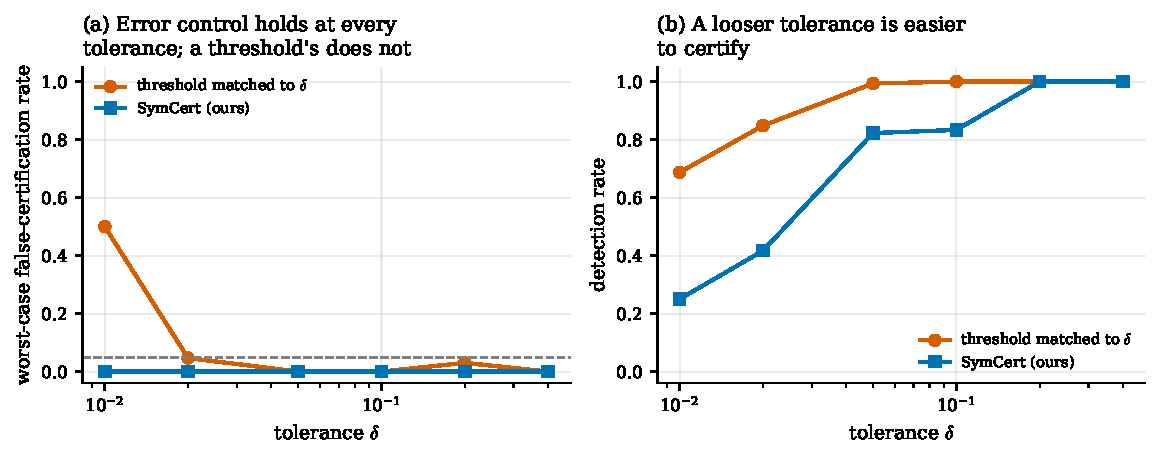
\includegraphics[width=0.78\textwidth]{../figures/fig7_tolerance.pdf}
\caption{Sweeping the tolerance, on a smaller grid: six systems, two sample
sizes, two noise levels. \textbf{(a)} \symcert{}'s worst-case
false-certification rate is zero at every tolerance; the threshold rule matched
to the same $\delta$ exceeds the nominal level at the tightest one and happens
to stay below it at the rest --- on the full grid of \Cref{tab:calibration} it
does not. \textbf{(b)} The tolerance is a real choice rather than a nuisance
parameter: it is the approximation the user is willing to accept, and accepting
more of it makes symmetry easier to certify, from a detection rate of $0.25$ at
$\delta=0.01$ to $1.00$ at $\delta=0.2$.}
\label{fig:tolerance}
\end{figure}

\subsection{Noise, coverage, and the model class}
\label{sec:coverage}\label{sec:modelclass}

\Cref{fig:mechanisms} isolates the four candidate mechanisms.

\paragraph{Noise is not the culprit.} With the model class correct and the data
covering the target domain, the threshold rule's errors are almost all missed
detections. We push this deliberately hard: four systems with no symmetry, noise
levels from $0.1$ to $1.0$, sample sizes from $30$ to $400$, $500$ replications
per cell --- $32{,}000$ in all. The median smallest plug-in defect \emph{rises}
with the noise, to $1.64$ times its true value at noise level $1.0$, and across
all $32{,}000$ replications the smallest value ever observed was $0.066$, still
above the tolerance. This confirms the upward bias argued in
\Cref{sec:noise-theory}: additive noise on the right-hand side inflates the
numerator of the defect relative to a true symmetry, so it removes symmetries
rather than inventing them.

\paragraph{Coverage.} We shrink the region the data occupy from the full target
box to a box of $0.15$ times the half-width, keeping $N=2000$ and noise level
$0.02$, and run the nullspace computation on the empirical measure of the data ---
what one does when the sample is taken to stand for the domain of interest.
\Cref{fig:headline}(b) plots the false-certification rate against the
extrapolation bound $\sqrt{\kappa\kappa'}$ divided by the value
$\defect^\star/\delta$ it must reach for a spurious symmetry to be possible at
all, from \eqref{eq:kappacrit}. Of the $50$ settings, $13$ fall in the region
where \Cref{prop:kappa} \emph{proves} that no spurious symmetry can occur, and
in all $13$ the observed rate is exactly zero; of the $37$ beyond it, $14$ do
produce false certifications, rising to a rate of $1.0$. \symcert{}, which
measures the defect on the target domain and inherits the design's uncertainty
through $\hat\Sigma$, never certifies falsely and
instead reduces its certified dimension to zero as coverage degrades: on the
Hopf system it certifies the true one-dimensional algebra when the data cover
the domain and certifies nothing once the data occupy less than half of it.

\Cref{tab:trajectory} shows what the diagnostic says about trajectory data, the
way such data actually arrive. A single trajectory of the Hopf system converges
to the unit circle, an algebraic curve, so some bracket vanishes on the data
exactly and the extrapolation factor is infinite: a defect measured on those
points constrains nothing on the target domain, and any tolerance whatever can be
met there by a generator that is not a symmetry. Eight trajectories bring the
factor down to $24$ and a uniform design to $1.1$. In these particular runs the
nullspace rule happens to give the right dimension on every row --- these are
single realisations, not rates --- but on the single Hopf trajectory it does so
without support from the data, and \symcert{} correctly declines. The
corresponding rates, and the failures, are in \Cref{fig:headline}(b).

\begin{table}[t]
\centering\small
\begin{tabular}{llrrrrr}
\toprule
system & design & points & $\sqrt{\kappa\kappa'}$ & true dim.\ & nullspace dim.\ & \symcert{} dim.\ \\
\midrule
Van der Pol & single trajectory & 3000 & 34.9 & 0 & 0 & 0 \\
Van der Pol & 8 trajectories & 3200 & 9.7 & 0 & 0 & 0 \\
Van der Pol & uniform design & 3000 & 1.1 & 0 & 0 & 0 \\
Hopf & single trajectory & 3000 & $\infty$ & 1 & 1 & 0 \\
Hopf & 8 trajectories & 3200 & 24.0 & 1 & 1 & 1 \\
Hopf & uniform design & 3000 & 1.1 & 1 & 1 & 1 \\
Lorenz & single trajectory & 3000 & 231.3 & 0 & 0 & 0 \\
Lorenz & 8 trajectories & 3200 & 84.4 & 0 & 0 & 0 \\
Lorenz & uniform design & 3000 & 1.1 & 0 & 0 & 0 \\
\bottomrule
\end{tabular}
\caption{Trajectory data. A single trajectory that settles onto an attractor
gives an infinite or large extrapolation factor: the data lie in, or near, the
zero set of a possible bracket, so a defect measured on them says little about
the target domain. \symcert{} declines to certify exactly there.}
\label{tab:trajectory}
\end{table}


\paragraph{The model class dominates.} Fitting a class too small to contain the
truth is the strongest mechanism we found, and the only one that defeats
\symcert{} as well. Fitting a linear or quadratic model to a cubic system
produces a fitted field with symmetries the system does not have --- a linear
system always has an $n$-dimensional symmetry algebra --- and both the threshold
rule and \symcert{} certify them in up to $100\%$ of replications
(\Cref{fig:mechanisms}, third group). This is not a failure of the certificate
but of assumption (A1), and we report it as such. A lack-of-fit $F$-test against
the correct class rejects in $100\%$ of replications in every truncated setting
we ran; gating certification on it returns the false-certification rate to zero
without affecting the correctly specified settings.

The same failure arises without anyone choosing to truncate. Sequentially
thresholded least squares, the sparse regression at the core of data-driven
model discovery \citep{brunton2016discovering,champion2020unified,
kaptanoglu2022pysindy} and the object of its own convergence theory
\citep{zhang2019convergence}, deletes small coefficients. On a Hopf
normal form perturbed by a symmetry-breaking term of size $\varepsilon$, whose
rotation defect is $0.064$ at $\varepsilon = 0.1$ --- above the tolerance --- a
sparsity threshold of $0.25$ deletes the breaking term and reports an exact
rotational symmetry in $100\%$ of replications, against $17\%$ with no
thresholding. Certifying from the unpruned least-squares fit gives zero.
Sparsification and symmetry discovery interact, and the interaction is invisible
if the two steps are run in sequence without accounting for the first.

\subsection{How small a violation can be certified}
\label{sec:resolution}

\Cref{fig:headline}(c) tracks the certified tolerance on the one-parameter family
$F_\varepsilon = $ Hopf $+\ \varepsilon x^2 \partial_x$, whose rotation defect
grows continuously from zero. Over two decades of $N$ and three noise levels the
certified tolerance follows the $\sigma/\sqrt N$ scaling of the Le~Cam bound of
\Cref{prop:lecam}, exceeding it by a factor $8.1$, $8.3$ and $8.8$ at noise
levels $0.03$, $0.1$ and $0.3$ --- essentially constant, so the achieved rate is
optimal and only the constant is lost. \Cref{sec:tightness} measures the part of
that constant that is ours rather than the bound's.

The same experiment measures the opposite claim. At $N=1600$ and noise level
$0.1$, the lower certificate rules out exact symmetry ($L > 0$) for $49.5\%$ of
replications when the true rotation defect is $0.013$ and for $100\%$ when it is
$0.032$; when the system really is symmetric it does so in $1.0\%$ of
replications, against the nominal $5\%$.

\subsection{Problem dimension, and whether to split the sample}
\label{sec:dimension}

The width of the simultaneous certificate is governed by the number of model
coefficients $Q$, through the radius of the confidence ellipsoid; the width of
the split-sample pointwise bound is governed by an effective dimension of the
generator being tested, but it sees half the data. \Cref{fig:power}(b,c) settles
which wins: \textbf{the simultaneous certificate is narrower in all nine
configurations}, by factors of $1.4$ to $2.6$, and its detection rate is higher
in all nine. Sample splitting --- the standard remedy for the selection effect,
and one of the two remedies most often suggested for this problem --- is
counterproductive here, because the selection effect it protects against is
already handled for free by simultaneity.

The reason is visible in \Cref{sec:resolution}'s data. For a generator fixed in
advance --- where splitting is unnecessary --- the pointwise bound is never more
than $5\%$ narrower than the simultaneous one, and at small samples it is up to
$1.9$ times \emph{wider}, because the Gaussian-concentration bound it rests on
is loose there. Simultaneity over the entire candidate space is therefore
essentially free for this functional, while splitting costs the usual
$\sqrt{2}$ in effective sample size.

Two further readings. Increasing the \emph{candidate generator} class is nearly
free: moving from the $6$-dimensional affine class to the $12$-dimensional class
of all quadratic generators on the Hopf system changes the median certified
tolerance from $0.0464$ to $0.0457$. Increasing the \emph{model} class is not:
raising the polynomial degree from $3$ to $5$ ($Q$ from $20$ to $42$) widens it
from $0.046$ to $0.129$. The asymmetry is useful --- search widely over
generators, and spend your sample-size budget on the model class.

\begin{figure}[t]
\centering
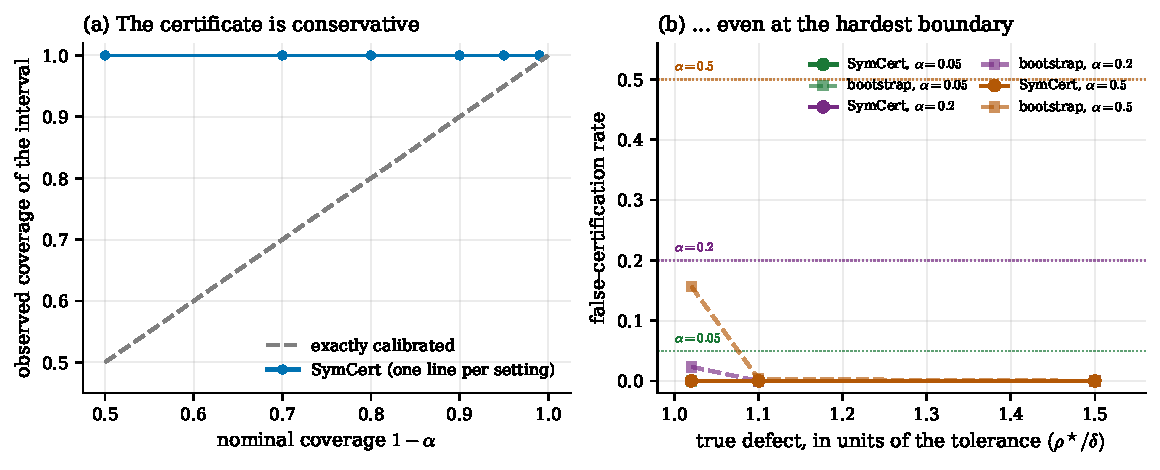
\includegraphics[width=0.78\textwidth]{../figures/fig4_tightness.pdf}
\caption{\textbf{(a)} Observed coverage of the certificate interval against its
nominal level, one line per setting. The certificate over-covers: the bound
treats numerator and denominator separately over the whole confidence ellipsoid.
\textbf{(b)} The deliberately hardest case: a system whose true defect sits just
above the tolerance, observed at the sample size that puts the median certified
bound exactly at the tolerance. \symcert{} (solid) never certifies falsely; a
calibration-targeting bootstrap (dashed), which has no finite-sample guarantee,
does.}
\label{fig:tightness}
\end{figure}

\begin{figure}[t]
\centering
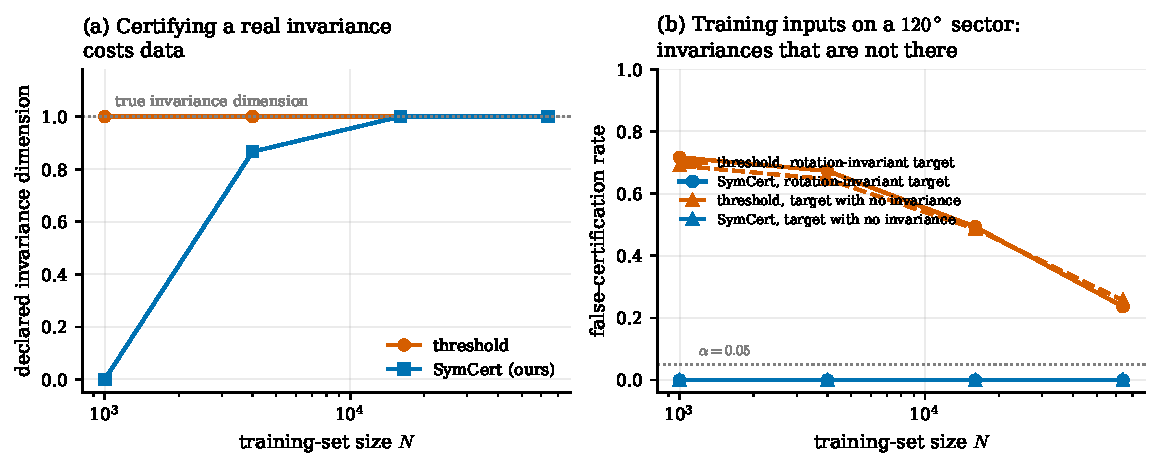
\includegraphics[width=0.78\textwidth]{../figures/fig5_invariance.pdf}
\caption{Invariances of a learned model rather than of a dynamical system.
\textbf{(a)} With training inputs covering the disc, both rules eventually
recover the one-dimensional rotational invariance of the target; certification
costs roughly sixteen times more data at this noise level. \textbf{(b)} With
training inputs confined to a $120^\circ$ sector, the fitted model is
unconstrained elsewhere, and the threshold rule declares invariances of the
target that the target does not have --- for both an invariant and a
non-invariant target. \symcert{} declines.}
\label{fig:invariance}
\end{figure}

\begin{figure}[t]
\centering
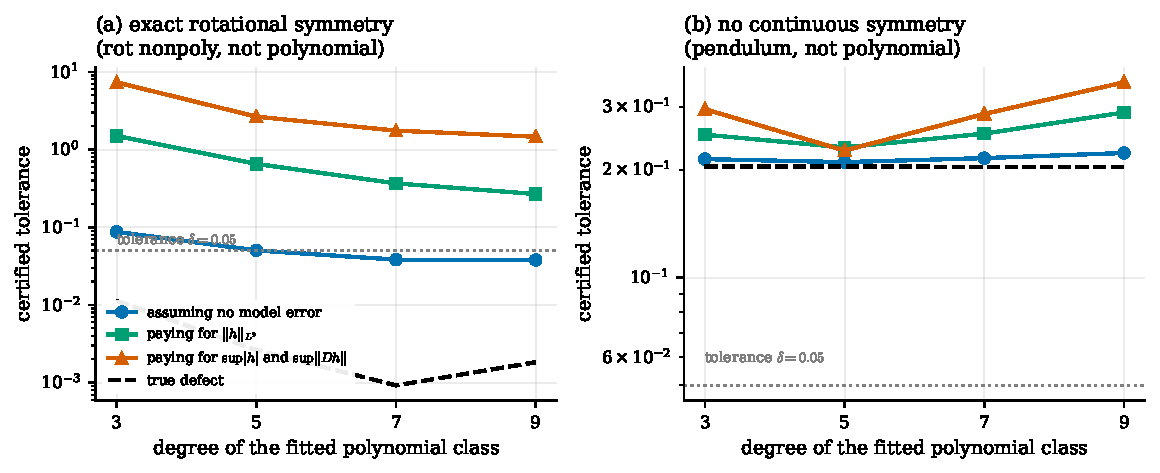
\includegraphics[width=0.78\textwidth]{../figures/fig6_modelerror.pdf}
\caption{Certifying a system that is not in any polynomial class. Ignoring the
approximation error (blue) gives a bound that is not valid; paying for it in
supremum norm (orange) is valid but vacuous; paying for it in $L^2$ against a
richer polynomial class (green) is valid and several times tighter, and improves
as the fitted class grows --- but on the left-hand system it is still above the
tolerance at degree $9$, so the exact rotational symmetry that is really there
cannot be certified honestly at this sample size. The dashed line is the true
defect, obtained by Monte-Carlo integration of the analytic bracket; the dotted
line is the tolerance $\delta = 0.05$.}
\label{fig:modelerror}
\end{figure}

\subsection{Is the guarantee tight?}
\label{sec:tightness}

A certificate that certified nothing would also never certify anything false.
\Cref{fig:tightness} shows that ours is conservative but not vacuous.
Panel (a): the interval covers the true defect more often than its nominal level
requires --- the observed coverage is $1.000$ at every nominal level from $0.50$
to $0.99$ --- because \eqref{eq:U} bounds numerator and denominator separately
over the whole ellipsoid. Panel (b) constructs the worst case deliberately: a
system whose true defect is $(1+\tau)\delta$ for $\tau$ as small as $0.02$,
observed at the sample size that puts the median certified bound exactly at
$\delta$. Across nine such configurations and $2{,}700$ replications the
false-certification rate is $0$.

To quantify the slack, we compare against a calibration-\emph{targeting}
alternative in the spirit of the parametric bootstrap
\citep{efron1979bootstrap}: draw $\beta^* \sim N(\bhat, \hat\Sigma)$ and take
the $(1-\alpha)$ quantile of $\defect(\theta;\beta^*)$. This has no finite-sample
validity, and in the boundary configuration it does certify falsely --- at rate
$0.157$ at $\alpha = 0.5$ and $0.023$ at $\alpha = 0.2$. Its intervals are
$9\%$ to $18\%$ narrower than ours. That is the measurable price of exactness on
this problem: between a tenth and a fifth of the width.

\subsection{Departures from the assumptions}
\label{sec:robustness}

\begin{table}[t]
\centering\small
\begin{tabular}{llrrr}
\toprule
& & \multicolumn{2}{c}{worst coverage} & worst false \\
\cmidrule(lr){3-4}
error distribution & design & exact Gaussian & sandwich & certification \\
\midrule
Gaussian & i.i.d.\ design & 1.000 & 1.000 & 0.000 \\
Gaussian, heteroskedastic & i.i.d.\ design & 1.000 & 1.000 & 0.000 \\
Laplace & i.i.d.\ design & 1.000 & 1.000 & 0.000 \\
Student $t_4$ & i.i.d.\ design & 1.000 & 1.000 & 0.000 \\
\midrule
Gaussian & trajectories, exact states & --- & 1.000 & 0.000 \\
Gaussian & trajectories, noisy states & --- & 1.000 & 0.000 \\
\bottomrule
\end{tabular}
\caption{Coverage of the certificate under departures from the homoskedastic
Gaussian model, at nominal $0.95$, over 24 design settings
and 24 trajectory settings. The certificate depends on the errors
only through a confidence ellipsoid for a least-squares estimator, and is
correspondingly insensitive to their shape and to dependence between rows. The
last block is the case the guarantee does \emph{not} cover: with noisy states and
differenced derivatives the regressors carry error, and coverage held here only
because the resulting bias happens to inflate the defect
(\Cref{sec:robustness}).}
\label{tab:robustness}
\end{table}


\Cref{tab:robustness} reports coverage under errors that are Student-$t_4$,
Laplace, or heteroskedastic, with the exact Gaussian ellipsoid and with a
sandwich covariance \citep{white1980heteroskedasticity}, and under trajectory
data where the rows are strongly dependent. Coverage never falls below nominal
in any of the $48$ settings, and no false certification occurs in any of them.
The certificate is not fragile to the shape of the error distribution, because
it depends on the errors only through a confidence ellipsoid for a least-squares
estimator.

The assumption that does bind is that the \emph{states} are observed without
error. We test it on trajectory data --- twelve solution segments per replication,
so the rows are strongly dependent as well --- in two modes: exact states with
noisy right-hand sides, and noisy states with derivatives taken by central
differences. With exact states the certified dimension on the Hopf system is
$1.00$ at state-noise level $0.01$ and $0.98$ at $0.05$. With noisy states it is
$0.07$ and $0.09$: the errors-in-variables bias attenuates the fitted
coefficients, which inflates the defect and destroys detection. Coverage held at
$1.0$ in all $24$ trajectory settings, but that is a property of this particular
attenuation acting in the conservative direction, not a guarantee. For that regime the honest options are the weak or
integral formulation of model discovery \citep{messenger2021weak}, ensemble
resampling of the fit \citep{fasel2022ensemble}, or an explicit
errors-in-variables treatment; we do not claim validity there.

\Cref{fig:modelerror} completes the picture for genuinely non-polynomial
systems, and it is the least comfortable result in the paper. On a
non-polynomial planar flow that has an exact rotational symmetry, a degree-$5$
fit gives a certified tolerance of $0.050$ if model error is ignored, $0.65$ if
it is paid for in $L^2$ against a degree-$9$ class, and $2.65$ if it is paid for
in supremum norm --- the last two both vacuous. Raising the fitted degree to
$9$ shrinks the measured relative $L^2$ model error to $0.5\%$ and the certified
tolerance to $0.27$, still too wide to be useful. The reason is the derivative
amplification noted in \Cref{sec:modelerror}: the bracket differentiates, so the
constant converting a bound on $\|h\|$ into a bound on $\|[\xi,h]\|$ grows with
the degree of the class $h$ is allowed to occupy, and it grows faster than the
approximation error falls.

On the damped pendulum, which has no continuous symmetry, the same accounting is
cheap --- true defect $0.204$, certified bounds between $0.21$ and $0.35$ across
all four degrees and both forms --- because a degree-$5$ polynomial reproduces
$\sin$ on the target domain to a relative $L^2$ error of $0.07\%$. Note also that
the model error is not monotone in the degree: at degree $9$ the fit is
ill-conditioned enough that both $\eta_0$ and $\eta_2$ increase again. The
practical rule of \Cref{sec:modelerror} therefore needs one qualification:
enlarge the model class until a lack-of-fit test is satisfied, and no further.

\subsection{Scaling with the state dimension}
\label{sec:scaling}

The state dimension enters twice: through the number of model coefficients $Q$,
which sets the radius of the confidence ellipsoid, and through the number of
candidate generators $P$, which sets how many directions are searched. Only the
first should matter, and \Cref{tab:scaling} bears that out. On linear systems in
$n = 2,\dots,6$ built from rotation blocks --- whose symmetry algebra is the
commutant of the coefficient matrix, of dimension $n$ --- false certification is
zero in all $20$ cells while the search space $P = n^2$ grows from $4$ to $36$.
What the growth costs is width: at $N = 12800$ the certified tolerance rises
from $0.0017$ at $n=2$ ($Q=6$) to $0.0050$ at $n=6$ ($Q=42$), a factor $2.9$
against the $\sqrt{Q}$ prediction of $2.6$. The whole $n$-dimensional algebra is
recovered in every replication from $N = 800$ at $n = 4$ and from $N = 3200$ at
$n = 6$. One certificate costs between $0.015$ and $0.031$ CPU-seconds across this range,
dominated by the $O(Q^3)$ eigendecomposition inside the trust-region solves.

\begin{table}[t]
\centering\small
\begin{tabular}{rrrrrrrr}
\toprule
$n$ & $P$ & $Q$ & true dim.\ & \multicolumn{3}{c}{certified tolerance (median)} & CPU-s / cert.\ \\
\cmidrule(lr){5-7}
 & & & & $N{=}800$ & $N{=}3200$ & $N{=}12800$ & \\
\midrule
2 & 4 & 6 & 2 & 0.0072 & 0.0036 & 0.0017 & 0.015 \\
3 & 9 & 12 & 3 & 0.0110 & 0.0054 & 0.0027 & 0.017 \\
4 & 16 & 20 & 4 & 0.0122 & 0.0069 & 0.0031 & 0.019 \\
5 & 25 & 30 & 5 & 0.0194 & 0.0097 & 0.0048 & 0.024 \\
6 & 36 & 42 & 6 & 0.0210 & 0.0108 & 0.0050 & 0.031 \\
\bottomrule
\end{tabular}
\caption{Scaling in the state dimension, on linear systems whose symmetry
algebra is the commutant of the coefficient matrix. The candidate search space
$P = n^2$ grows quadratically with no cost to validity; what costs is the model
class $Q$. False certification was zero in all 20 cells.}
\label{tab:scaling}
\end{table}


\subsection{A case study on real measurements}
\label{sec:realdata}

The Hudson's Bay Company lynx and hare pelt records for 1900--1920 are the
canonical real data for two-dimensional predator--prey model discovery: $21$
annual counts, from which central differences give $19$ usable
state--derivative pairs. Fitting a quadratic vector field and running the
pipeline gives the plug-in defect spectrum
$(0.18,\ 0.33,\ 0.68,\ 1.17,\ 1.31,\ 1.40)$, an extrapolation factor
$\sqrt{\kappa\kappa'} = 58$, and a smallest certified tolerance of $2.3$ ---
larger than the largest value the defect can take. \textbf{With nineteen
observations, no symmetry claim of any kind is supported.} The plug-in spectrum
nonetheless \emph{looks} informative, and at a tolerance of $0.3$ --- not an
unreasonable choice --- a threshold rule would report a one-dimensional symmetry
algebra.

This is the honest outcome, and it is the one we would want a method to produce.
We present it as a case study rather than as a validity claim: derivatives
differenced from noisy annual counts put error in the regressors, which
(\Cref{sec:robustness}) is the departure our guarantee does not cover.

\subsection{Invariances of a learned model}
\label{sec:invariance}

The same machinery applies where $F$ is a learned function and $\xi$ generates
an invariance: the Lie derivative becomes $\nabla f \cdot \xi$, and the defect
becomes the root-mean-square cosine of the angle between the model's gradient and
the generator, again a ratio of norms of linear images of the coefficients. We
fit degree-$6$ polynomial regressions to noisy samples of three planar targets --- a
rotation-invariant one, three that are invariant only up to a controlled amount,
and one that is not --- and ask which invariances \emph{of the target} may be
declared. \Cref{fig:invariance} reports the result. With the training inputs
covering the disc, both the threshold rule and \symcert{} recover the
one-dimensional invariance once $N$ is large enough, \symcert{} requiring
roughly $16$ times more data at noise level $0.05$. With the training inputs
covering a $120^\circ$ sector, the threshold rule declares invariances that the
target does not have, at rates up to $0.76$, for both an invariant and a
non-invariant target; \symcert{} never does.

This is a second and distinct coverage mechanism, and it completes the picture of
\Cref{sec:coverage}. There the \emph{integral} was extrapolated: the Gram matrix
computed on the data stood in for the one on the target domain, and $\kappa$
measured the gap. Here the integral is exact and the \emph{model} is
extrapolated: outside the sector the fit is unconstrained, and it drifts toward
functions that happen to look invariant. No diagnostic on the states alone can
see this. \symcert{} does, because the same lack of constraint that lets the fit
drift also inflates $\hat\Sigma$ in exactly those directions, and the
certificate is then too wide to clear any useful tolerance.
